\chapter{Emperical Evaluation}
\label{chap:evaluation}

We created several experiments in order to provide a thorough comparison of online versus offline learning as well as CPU versus GPU processing. The opening section of this chapter provides technical information on how we implemented the different algorithms used in the Quake III environment. The remainder of the chapter will contain detailed explanation of each experiment we ran, including why we ran the experiment, the environment setup, and a discussion of the results.

\section{Quake III Bots}

The source code for Quake III is available on github under an open source license. \cite{q3code} Included with the source code is a Visual Studio solution file for C compilation. To perform the experiments we implemented LSPI using CUDA acceleration in a C++ project and then integrated this code into the Quake III source code.

The Quake III solution is separated into multiple projects representing different parts of the game engine and implementation; for our work we only modified the \emph{game}, \emph{botlib}, and \emph{server} projects, with most of the work occuring in the \emph{game} project. Modifications to \emph{botlib} were required to allow our bots to peak into the state of the environment without affecting it, which caused bugs when our bot checked the state of the environment more frequently than the native bots. The modifications to \emph{server} were only to facilitate the changes in \emph{botlib}.

Recall from the background section that the Quake III AI is separated into four levels which are further broken into subsections. The \emph{botlib} provides the implementation for most of the lower two levels. The remaning logic is contained in the \emph{game} project, including the AI Network which guides actions at a high level. Our bot was implemented largely by supplanting the AI Network's finite state machine and allowing more frequent and flexible state transitions.

\subsection{Understanding the AI Optimizations}

Generic AI systems generally function on the assumption that we alternate between a few states: environment observation, action selection, action execution, and reward collection. With this flow it is very easy to change AI implementations by simply taking the environment observations and replacing the action selection step. However, in a performance constrained environment it is generally considered expensive and unnecessary to follow this flow.

Suppose we had an agent acting in the Quake III environment called Cindy. Cindy's first action (as with every Quake III bot) is to search for a long-term goal. This can be an item or an area on the map. Because Cindy already has some knowledge about the arena, she decides she wants to go to the other side of the map and pick up her favorite gun, the BFG. However, before she moves forward she looks around at the nearby items. Since there are only other weapons and no armor, and Cindy \emph{really} loves the BFG, she decides to just head toward her current long-term goal.

After Cindy takes a step the world moves forward a step as other agents in the environment take similar actions. Now Cindy has the choice to re-evaluate her decision, but should she? After all, she just took a full profile of her environment and selected her choices, with little to no environmental changes occurring. It is very likely that Cindy would just make the same decision again and it takes much less thought to re-evaluate the environment.

Once again, Cindy takes a step and the world move forward. This time; however, an enemy has become visible. Even though Cindy only decided on her current task two steps ago, she decides to change her goal to killing the enemy. Notice that Cindy did not reconsider her entire environment: she could have realized that the starting weapon was not a good choice to attack her enemy with, resulting in turning around to grab a nearby weapon. Instead, Cindy only evaluates some small portion of her environment at each step and unless something critical in that portion changes, such as an enemy appearing, she will continue assuming the last decision she made was valid.

Cindy's behavior essentially represents the logic that the native Quake III bots follow. This performance optimization was critical for allowing several bots to fight in a match when desktop processors were still under the $1GHz$ limit and universally constrained to a single core. Unfortunately, this highly tangled system makes integrating a new bot very difficult. The next section discusses how we modified the AI structure to support a more traditional model for our own bots while still sharing code with the native bots.

\subsection{Using the Finite State Machine}

The existing finite state machine code is separated into two types of methods: transition methods and node execution methods. The transition methods generally perform some minor tasks like print out chat responses or tracking the number of node transition the bot executes, and then it sets a \emph{AI node} function pointer to the node execution method for that specific transition. From Cindy's example, when the enemy appeared this would trigger a state transition by calling the \emph{battle fight} node transition function, called \emph{enter battle fight}. Before calling this function the AI node would be referencing the node \emph{seek long-term goal}, but after the transition function this would reference the node \emph{battle fight}.

Rather than limiting the bots to executing only a single node in any given game step, each node execution function returns \emph{true} when it has finished executing and \emph{false} if it has called a transition method to a node before it reached the end of the current node. This causes the code calling the nodes to continue calling until a node reaches completion.

\begin{algorithm}
\caption{Node Execution Method}
\label{ainode}
    {\fontsize{12}{10}\selectfont
    \begin{algorithmic}[1]
        \STATE Check for Special Nodes: \emph{Observer}, \emph{Intermission}, \emph{Dead}
        \STATE Ensure Movement Mode: \emph{swimming}, \emph{rocket jump}, \emph{etc}
        \STATE Execute Map Scripts
        \STATE Execute Node Scripts
        \STATE Setup Movement
        \RETURN \emph{true}
    \end{algorithmic}
    }
\end{algorithm}

Each execution node is formatted in the same way, following the pattern described in Algorithm \ref{ainode}. Intermixed among these primary steps are key conditionals which check portions of the state to see if a transition is necessary. If a transition is deemed necessary prior to step $5$, the node will return \emph{false}.

In order to utilize as much of node execution method as possible, our bot needed to do two things: skip any conditionals which could change state and execute any possible state changes when the first node is called each step. There are some exceptions to this rule required to maintain proper bot behavior. For example, there is a node called \emph{seek activate entity} which is used to open doors by shooting buttons. We did not want to modify this code as it could fundamentally break the bot's ability to navigate the map.

\begin{algorithm}
\caption{Modified Node Execution Method}
\label{ainode:custom}
    {\fontsize{12}{10}\selectfont
    \begin{algorithmic}[1]
        \STATE Check for Special Nodes: \emph{Observer}, \emph{Intermission}, \emph{Dead}
        \STATE Ensure Movement Mode: \emph{swimming}, \emph{rocket jump}, \emph{etc}
        \IF{Custom Bot and No Action Chosen}
            \STATE Observe Environment
            \STATE Get Action
            \IF{Bot Wants to Switch Nodes}
                \STATE Call Transition Method
                \RETURN \emph{false}
            \ENDIF
        \ENDIF
        \STATE Execute Map Scripts
        \STATE Execute Node Scripts
        \STATE Setup Movement
        \RETURN \emph{true}
    \end{algorithmic}
    }
\end{algorithm}

To achieve these goals we added a new flag called \emph{bottype} to the bot's personal state data. By default this value is $0$, so we used the values $1$ to represent LSPI agents and $2$ to represent gradient policy agents. Once we knew if a given bot was native or our own, we simply modified all of the nodes to ignore state transitions if it was our bot, and we added a new conditional demonstrated in steps $3-10$ of Algorithm \ref{ainode:custom}.

\subsection{Actions and Goals}

As our code was utilizing the AI Network's finite state machine, our code was also limited by the actions available in this state machine. The finite state machine contains twelve nodes total; however, half of the nodes are maintained for special scenarios including bot death and match intermissions. As a result there are only six nodes available, each of which maps to an action available to our agent. The resulting actions are as follows:

{\fontsize{12}{5}\selectfont
\begin{itemize}
    \item \emph{Seek Long-term Goal} - Selects an item or location across the entire map and attempts to reach that goal. After an extended period of time has passed the bot will re-evaluate its goal.
    \item \emph{Seek Nearby Goal} - Assumes a goal has already been selected and moves toward the goal. After a short period of time the bot will re-evaluate its goal.
    \item \emph{Battle Fight} - The enemy becomes the goal and the bot will attempt to do combat maneuvers while attacking the enemy.
    \item \emph{Battle Chase} - The bot will move toward the last known location of the enemy in an effort to catch and kill them.
    \item \emph{Battle Retreat} - The bot selects a goal far away and moves toward it in an attempt to flee from the battle.
    \item \emph{Battle Nearby Goal} - The bot selects a nearby item to improve its odds of defeating the enemy.
\end{itemize} }
Note that all of the actions prefixed \emph{Battle} are only valid if there is an enemy, and any actions without this prefix are only valid if there is no enemy.

As far as goal selection and seeking is concerned, our bots do not entirely follow the same rules as the native bots. In the default Quake III source code, attempting to find a nearby goal automatically updates the bot's goal state. In addition to this, selecting a goal creates sets a value referred to as an \emph{avoid timeout}. This value specifies a period of time during which the bot should ignore that goal, which means that any further searches before the timeout expires will skip that goal. 

Since our bot searches for goals every step, we had to modify the code to pass in a parameter specifying if we were trying to peek without changing the state. However, even this was not complete enough since the node \emph{seek nearby goal} does not actually search for nearby goals. As a result we had to modify the code to pick a nearby goal whenever attempting to transfer into that state. In addition, since the bots do not actually detect whether an item is present and we don't share the avoid scheme of the native bots, we modified the bots to add an avoid timeout to any item which they were potentially touching. The end result should be equivalent to the native bots; however, we did notice a few minor bugs where the bot ran out of available goals. Luckily this happens infrequently, is handled gracefully by the game (by resetting avoid timers), and is avoided by good policies.

Goal selection is a limiting factor for our bots: although we can direct the bot to look for a goal through the seeking and nearby goal states, we have no control over the goal selection itself. As a result, we rely completely on the Quake III AI implementation to decide what items our bot should pick up and whether the bot wants to roam or defend a key location. As a result, some of our results do not properly demonstrate the full capabilities of a machine learning AI in this environment; however, we were still able to create bots capable of repeatedly defeating the native bots.

\section{Performance Scaling}

The performance of the GPU on tasks which benefit from parallel processing is not always better than the CPU. Remember that the GPU processes single threads slower than the CPU and is constrained by memory operations. As a result, the GPU shows its greatest performance gains as the size of the input scales. In fact, current generation GPUs hit peak performance for matrix operations when the matrix dimensions are close to $1024 \times 1024$. \cite{cuda:perf} With that in mind we ran experiments to demonstrate the impact of this on LSPI as the size of the input scales.

There are two inputs for LSPI that scale, each of which we ran experiments to evaluate. The first experiment we ran tested the performance of LSPI as the number of samples to process increased. The experiment was setup by first collecting $150,000$ samples from an agent following a random policy with a $25\%$ exploration rate. We then seperated these samples into groups of varying size ranging from $30,000$ to $150,000$. With each group of samples we trained an agent using the GPU implementation and then using the CPU implementation and measured the amount of time it took to converge on a policy. For consistency both implementations were executing the same code on the same hardware with the exception of the BLAS calls, which were unique to the specific implementation. The GPU implementation was executed inside of the Quake III engine by halting all operations until a policy was generated. Due to technical limitations, the CPU implementation would not function in the Quake III engine; however, we were able to execute the same code path outside of the Quake III engine to ensure the results would be consistent. \footnote{TODO: I should put more information on the setup in the appendix.}

Figure \ref{fig:samples} shows the graph of our results complete with linear best-fit lines. \footnote{TODO: The raw data and fit analysis is available in the Appendix.} You'll notice that the GPU implementation not only performs worse than the CPU implementation, but also appears to scale worse with the number of samples. At first glance, this may seem contrary to the expectations of our work. In reality, these results are both reasonable and expected. In order to minimize the performance impact of the basis function we chose to run these tests with the smallest basis function, which had $30$ values. The result is that the largest matrix computation involves $30 \times 30$ or $90$ operations. A CPU is capable of processing this number of operations in a very short period of time, and does not have to do any memory copy operations before processing the samples. The GPU can compute most of these operations in parallel; however, first all of the samples must be copied from host memory to device memory. The end result is that with such a small basis the CPU performs better and because the GPU must always do a memory copy, the CPU also scales better.

\begin{figure}
	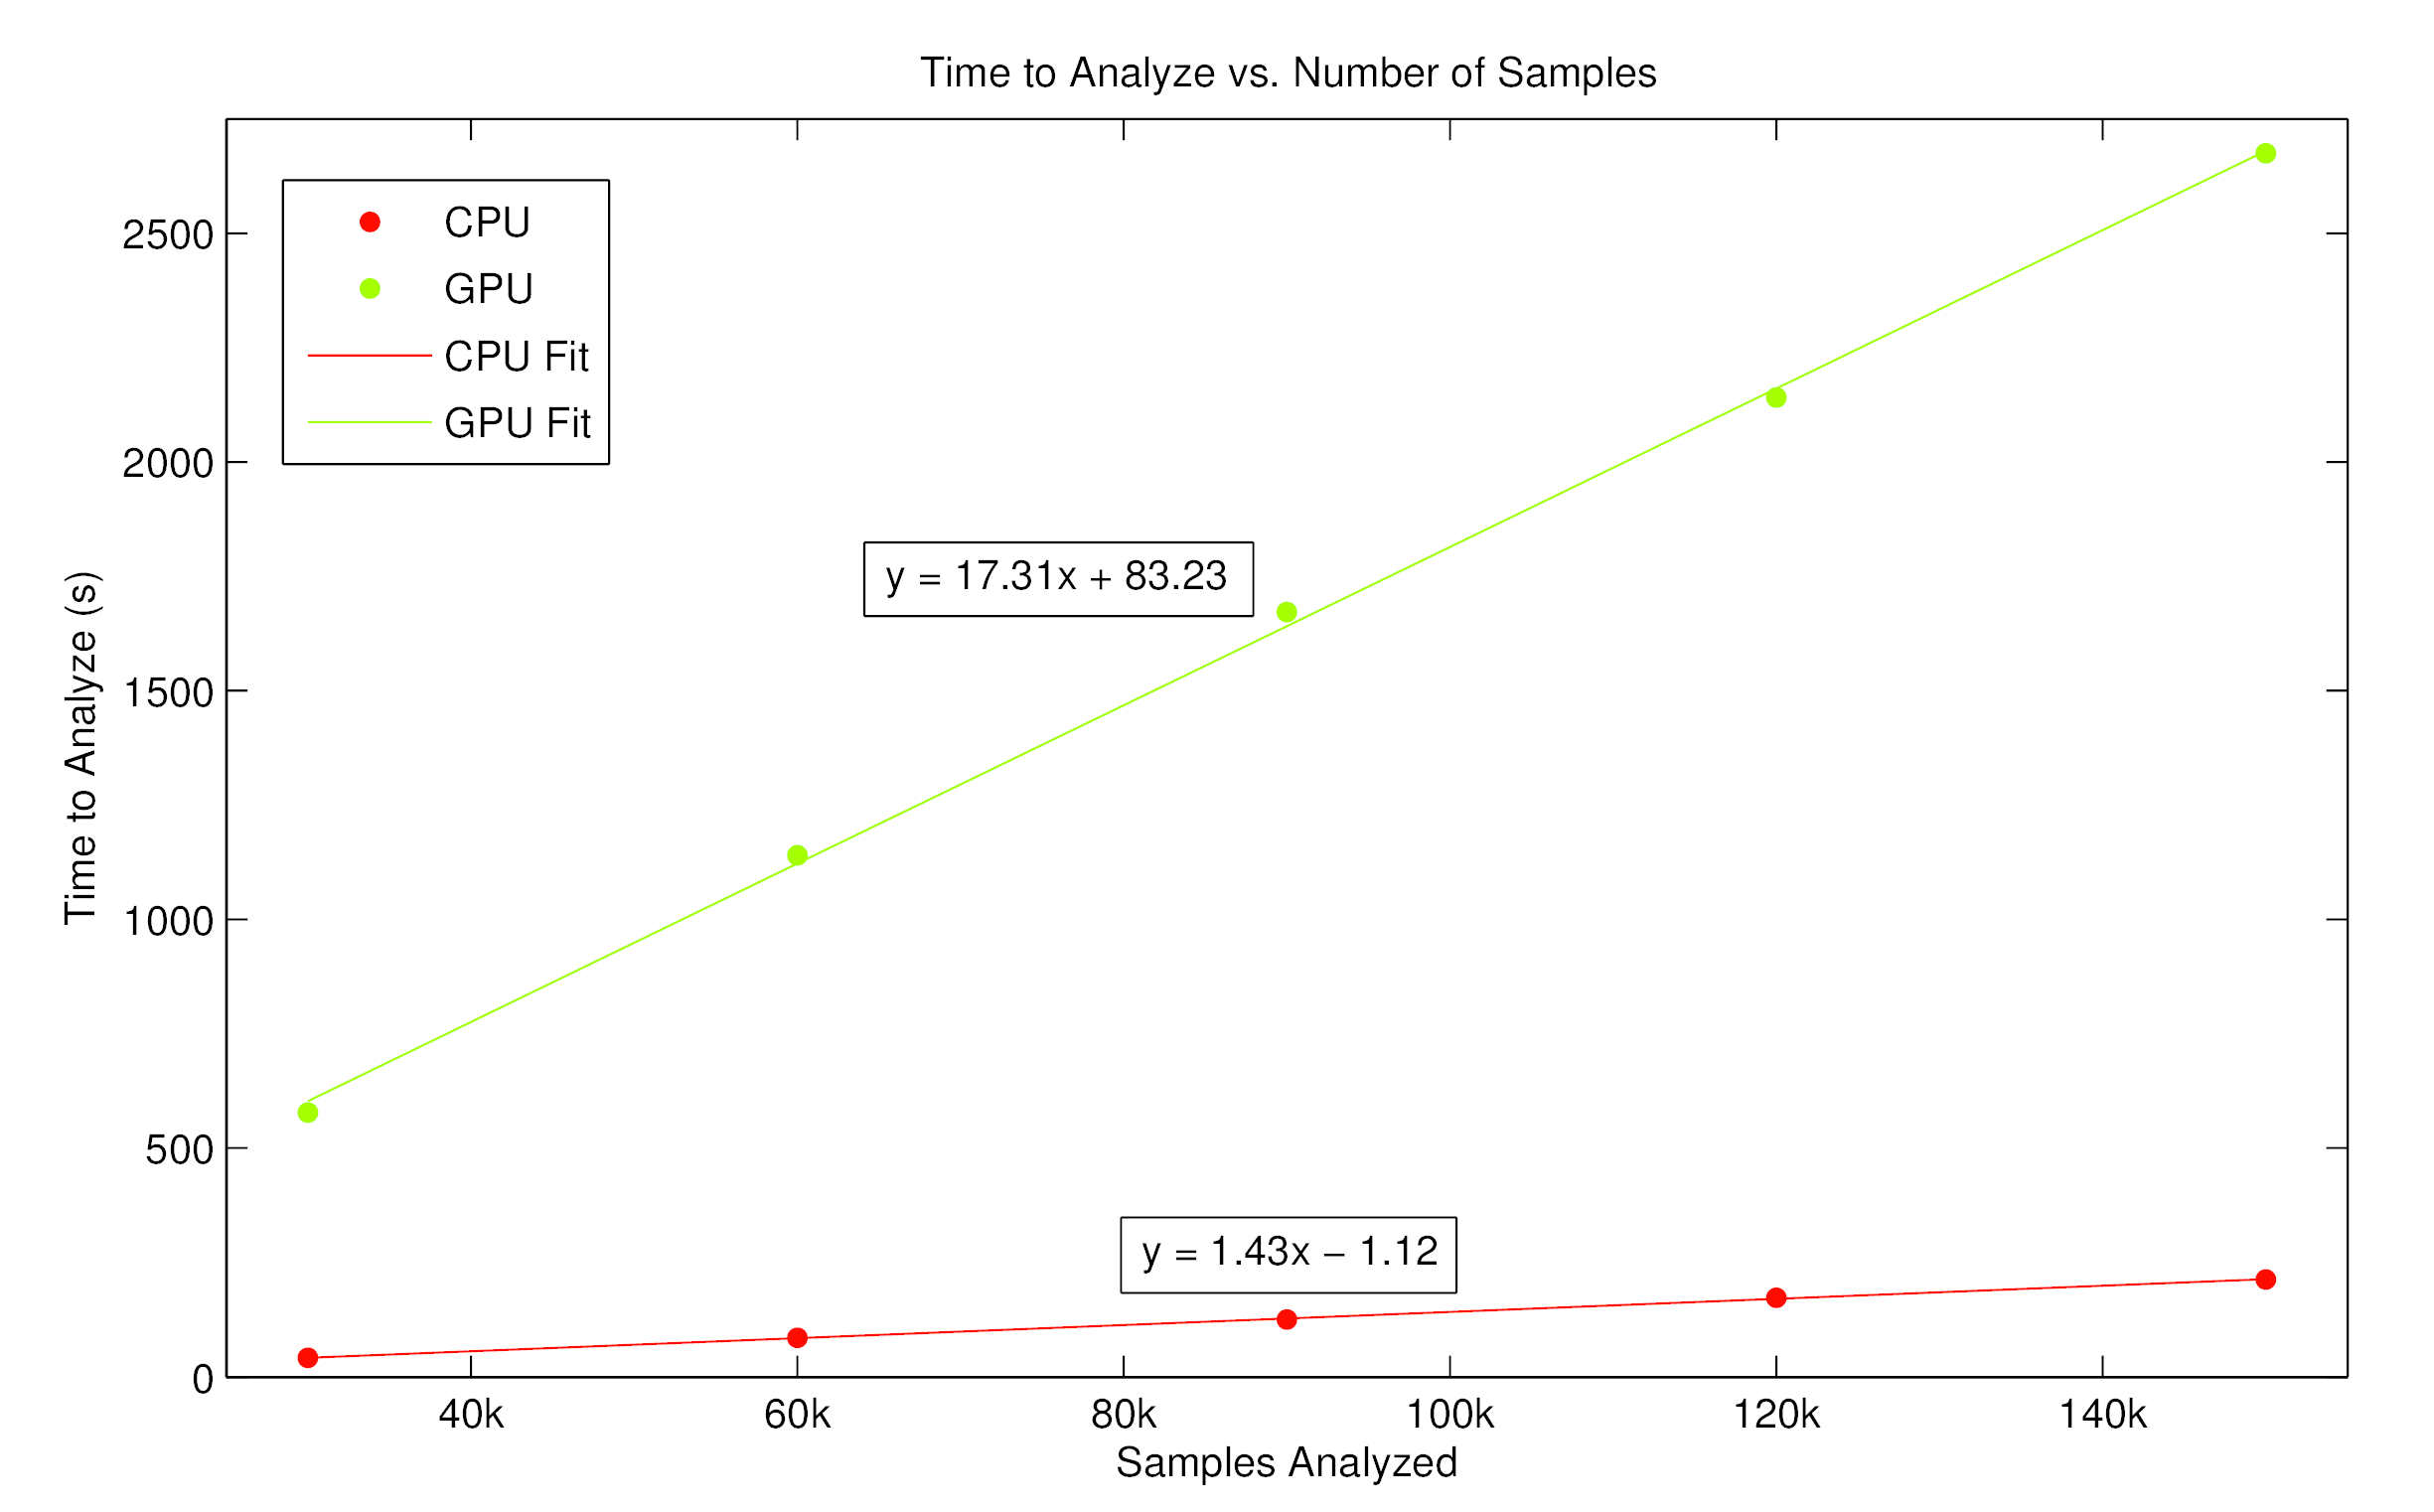
\includegraphics[width=\textwidth]{Time_vs_Samples.png}
    \caption{Plot of performance based on sample size}
	\label{fig:samples}
\end{figure}

The second experiment tested the performance of LSPI with a constant number of samples while the basis size increased. The experiment was setup by collecting $10,000$ samples from an agent following a random policy with a $25\%$ exploration rate. These samples were then used to train agents with basis functions which ranged in size from $30$ to $258$. As with the samples scaling experiment, every attempt was made to ensure these experiments were completed in identical environments. Due to the variance we witnessed in our experiments we repeated this training for each agent three times for both the CPU and GPU implementation. The results are graphed with fit lines in Figure \ref{fig:basis}. \footnote{TODO: Put the raw data and figure analysis.}

\begin{figure}
    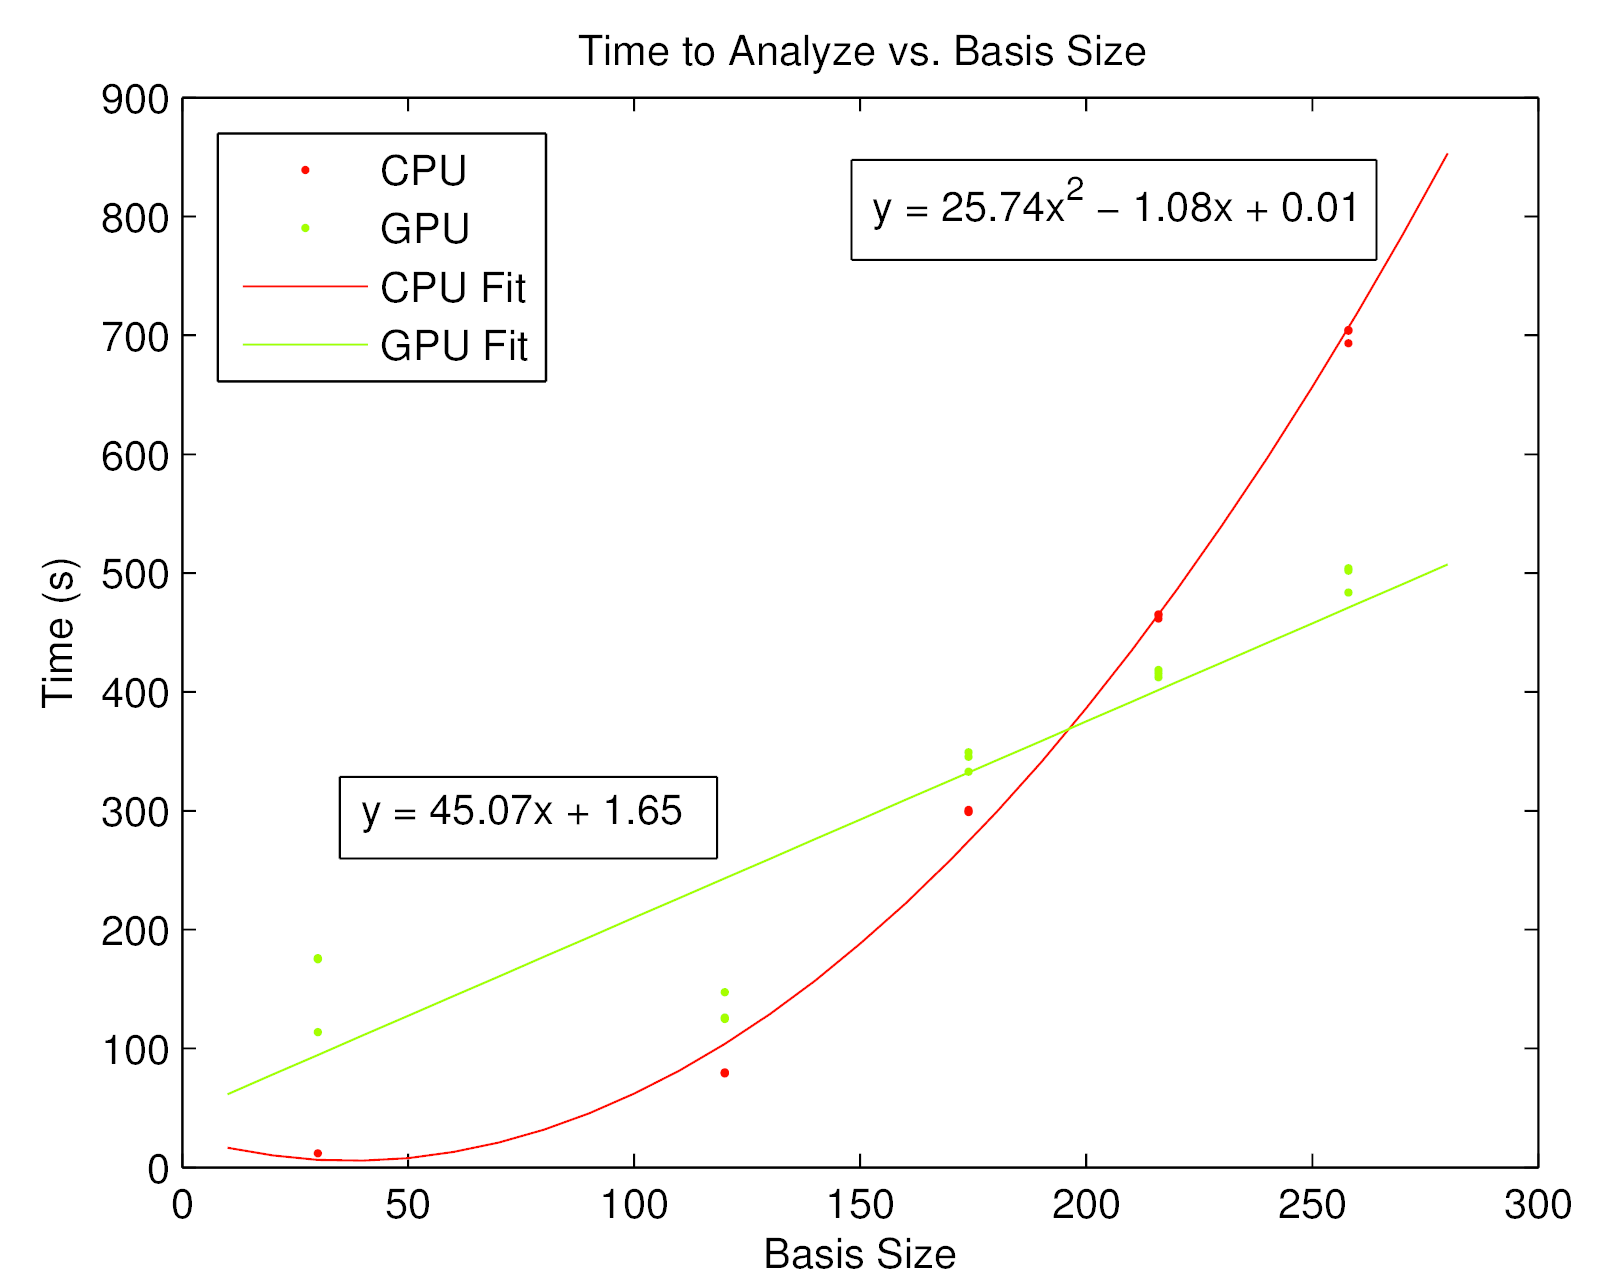
\includegraphics[width=\textwidth]{Time_vs_Basis.png}
    \caption{Plot of performance based on basis size}
    \label{fig:basis}
\end{figure}

Based on the data we collected, it is clear that while the GPU performs slower than the CPU with small basis sizes, the GPU scales well with increasing basis size. For our particular configuration the performance crossover occurs around $200$; however, that intersection point will vary based on the specific hardware configurations as well as the optimizations used to improve performance.

While the speeds we measured on the CPU were relatively stable, we noticed a high level of variance in our measurements for the GPU. Based on our knowledge of how linear algebra operations scale on the GPU, we would expect LSPI to scale approximately linearly on the GPU. Most of our data supports this; however, there are some outliers present on the graph.

When we measured the time to analyze the samples using a basis size of $120$ we were consistently seeing results that were comparable to the amount of time needed to analyze the samples using a basis of size $30$. To understand this result, we must first understand what factors will impact the amount of time needed to execute LSPI.

At its core, LSPI can be viewed as an optimization algorithm which iteratively executes the algorithm LSTD$Q$ in an attempt to locate the policy which maximizes the utility of the agent for the given samples. Depending on both the samples and the basis function used to evaluate the samples, the number of iterations of LSTD$Q$ necessary can change. Looking at Figure \ref{fig:basis} the data shows that although it is less noticeable, all three tests for the CPU also appear under the curve. This suggests that the particular features we selected may have had an impact on the number of iterations of LSTD$Q$ required to converge.

Another potential contributing factor to this result is the nature of the GPU architecture. When code is executed on the GPU, some number of processing units is allocated. The number of processing units allocated does not necessarily correspond with the size of the data input. As a result, there may be processing units which are effectively idle. The end result is that two operations with different input sizes may take the same amount of time. Between the architecture of the GPU and the interaction of the basis features with the speed of convergence, we feel that these results still fall within the expected range.

When it came time to plot fit lines for the data, the choice was obvious for the CPU: the results very clearly represent a second degree polynomial, with $R^2 = 0.99$. For the GPU the choice was less obvious, particularly since the outlier at $120$ made any fit difficult. We chose a linear fit because the data fits a linear model better with the outliers removed. The fit was less consistent for the GPU data with $R^2 = 0.7987$.

It is important to keep in mind that the point at which the GPU overtakes the CPU in performance will vary based on specific hardware configurations, as well as the level of optimization put into the implementation. As stated earlier, we chose to optimize very little to focus on the scaling performance gains. Futhermore, unless the CPU implementation was capable of being optimized at a rate much higher than the GPU optimizations, these performance tweaks would only serve to lower the barrier for seeing improvements with the GPU.

In our experiments we were able to generate very good policies with a very small basis function; however, this is largely due to the amount of hand written scripts our bot relies on to interact with the environment. While this allowed us to test the performance of LSPI under different conditions very well, our AI implementation does not do well at showcasing the benefits to AI design of machine learning algorithms. 

To understand the benefits of a large basis function, consider designing an AI agent for Quake III from the ground up. In order to manage the complexity of the environment, it is helpful to have some basic actions available to the agent: \emph{attack}, \emph{get health}, \emph{get weapon}, \emph{get armor}, \emph{get powerup}, \emph{search for enemy}, \emph{defend location}, \emph{flee from enemy}, \emph{change weapon}, \emph{reload}. Already our agent has more actions available than the implementation was used for testing.

Now that we have defined some actions for our agent, consider what information would be useful in order to make intelligent decisions. First and foremost, the agent needs information on its own state: \emph{health}, \emph{armor}, \emph{equipped weapon}, \emph{available weapons}, \emph{equipped ammo}, \emph{available ammo}. Keep in mind that some of these features, such as equipped weapon and available weapons, would need to be represented by multiple values in the basis. In fact, representing this information in Quake III would already result in a basis with $23$ values which must be repeated for each of the $10$ actions we have defined, and we still lack the information to make more complex decisions such as how to choose an area to defend.

Of course, the basis size can be made smaller by carefully controlling the basic actions available to the bot and carefully selecting features. However, the key result of this experiment is demonstrating that the advent of GPU acceleration enables an AI designer more control over selecting features and actions for an agent without suffering the significant performance degredation present with CPU based algorithms as the basis size increases.